% CHAPTER 02 - REFERENCIAL TEORICO

% \begin{itemize}
%     \item \add{Conceitos de SLAM, fusão sensorial, navegação autônoma e mapeamento em sistemas multirrobôs.}
%     \item \add{Revisão de abordagens em SLAM (incluindo técnicas baseadas em sensores visuais e inerciais) e da literatura sobre sistemas de referência como o OptiTrack.}
%     \item \add{Discussão sobre desafios e limitações dos algoritmos desenvolvidos do zero e as vantagens de se utilizar bibliotecas consolidadas no ROS.}
% \end{itemize}

\section{Modelagem e Controle de Robôs Móveis}

Para controlar um veículo móvel de forma autônoma é necessário entender a física inerente ao seu movimento e buscar maneiras de modelar matematicamente seu funcionamento. Isso implica que, para controlar a posição e velocidade de um robô móvel, é necessário obter o modelo matemático que descreve seu movimento no espaço tridimensional em que o movimento é realizado. Porém, existem diversos tipos de robôs e plataformas móveis, com configurações diferentes de rodas, geometria e design, o que resulta em características distintas de estabilidade, manobrabilidade e controlabilidade. A Figura \ref{fig:mobile_robot_types} mostra três exemplos de configurações comuns de robôs móveis: robôs omnidirecionais, que podem se mover em qualquer direção no plano; robôs diferenciais (também denominados de uniciclos) e os robôs tipo carro (\textit{car-like} em inglês), também conhecidos como robôs \textit{Ackerman}. Esta última configuração é menos comum em robôs móveis devido à sua manobrabilidade limitada, com exceção de robôs projetados para o sistema viário \cite{book:siegwart2011}.


% Figura dos tipos de robôs móveis
\begin{figure}[htb]
    \centering
    \caption{Tipos de Robôs Móveis Terrestres.}
    \label{fig:mobile_robot_types}

    \begin{subfigure}[b]{0.3\textwidth}
        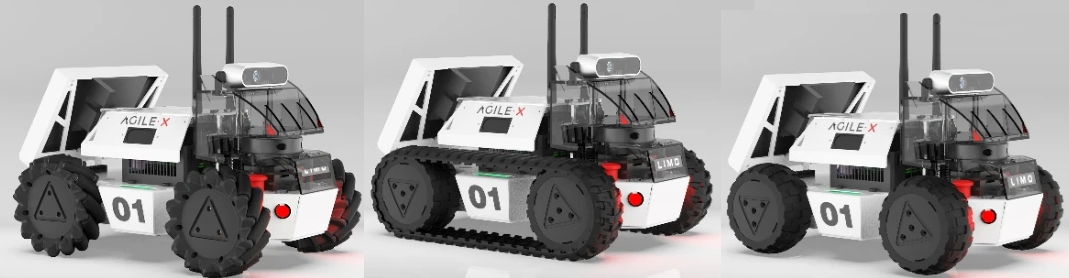
\includegraphics[trim=0 0 528 0, clip,  width=\textwidth]{img/Limo_modes.png}
        \caption{Robô Omnidirecional}
    \end{subfigure}
    ~
    \begin{subfigure}[b]{0.3\textwidth}
        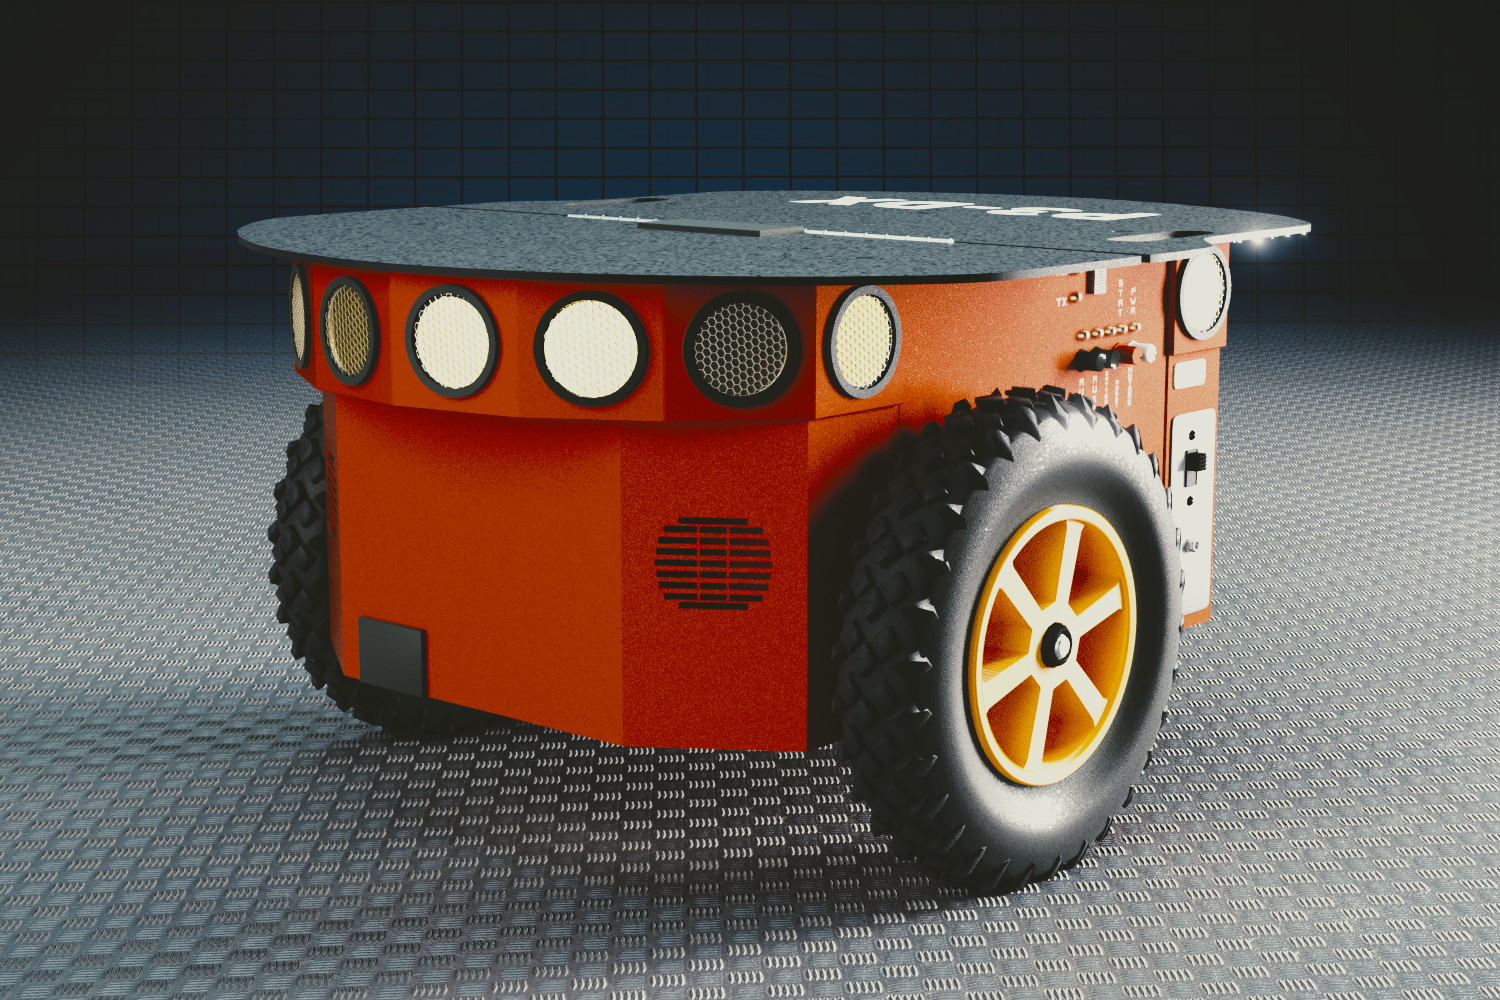
\includegraphics[width=\textwidth]{Pioneer 3-DX.jpg}
        \caption{Robô Diferencial Pioneer 3-DX}
    \end{subfigure}
    ~
    \begin{subfigure}[b]{0.3\textwidth}
        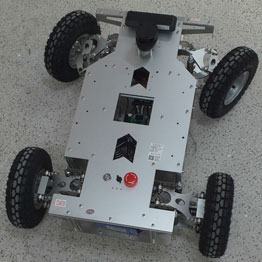
\includegraphics[width=\textwidth]{ackerman_robot.png}
        \caption{Robô Ackerman (\textit{car-like})}
    \end{subfigure}
    
    \sourceParbox[0.9\textwidth][\textbf{(a)} e \textbf{(c)}: \cite{Sarcinelli-Filho2023_2}; \textbf{(b)}: \cite{site:ArtStation_AynurZakirov}]
    % \source[\textbf{(a)} e \textbf{(c)}: \cite{Sarcinelli-Filho2023_2};\textbf{(b)} \cite{site:ArtStation_AynurZakirov}]
    % \note[0.8\linewidth][À esquerda, robô omnidirecional com rodas to tipo Mecanum e à direita robô diferencial (Uniciclo) Pioneer 3-DX]
\end{figure}


% >>> Comando para inserir a fonte em figuras <<<
% e.g.:
% \begin{figure}[!h]
%	\centering
%	\caption{Legenda da Figura.}
%	\includegraphics[width=0.7\textwidth]{figura.jpg}
%	\source[\citeonline{Referencia}.]
%	\label{fig:label_da_figura}
%  \end{figure}
%  
% Obs.: Se utilizar apenas "\source", será inserido
%       "Produção do próprio autor."

As plataformas móveis omnidirecionais são plataformas holonômicas (capazes de se mover em qualquer direção) e, portanto, não possuem restrições em seu sentido de movimento. Estas plataformas usam rodas projetadas especificamente para permitir movimentos nas direções transversais e longitudinais, permitindo que o robô obtenha velocidades em todas as direções do seu plano de trabalho (ver Figura \ref{fig:rodas_omnidirecionais}).

% incluir figura dos tipos de robos
\begin{figure}[htb]
    \caption{Rodas de Robôs Omnidirecionais}
    \centering    
    \begin{subfigure}[b]{0.2\textwidth}
        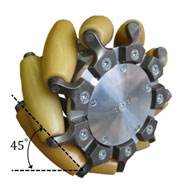
\includegraphics[width=\textwidth]{Omidirectional/omidirectional_robot_sarcinelli3.png}
        \caption{Roda Mecanum}
    \end{subfigure}
    \hspace{0.1\textwidth}
    \begin{subfigure}[b]{0.2\textwidth}
        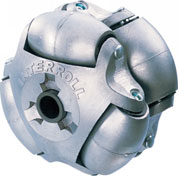
\includegraphics[width=\textwidth]{Omidirectional/omidirectional_robot_sarcinelli4.png}
        \caption{Roda \textit{Omni}}
    \end{subfigure}
    \source[Adaptado de \cite{Sarcinelli-FilhoControlRobots}]
    \label{fig:rodas_omnidirecionais}
\end{figure}


As plataformas móveis diferenciais são plataformas não holonômicas que contêm duas rodas principais, com motores independentes, responsáveis pelo movimento do robô. Geralmente, são equipadas com uma terceira roda, do tipo castor ou omnidirecional, para servir de apoio e manter o equilíbrio da plataforma.

Os robôs do tipo \textit{car-like} têm seu funcionamento semelhante ao dos carros utilizados no cotidiano, contando com uma plataforma com quatro rodas, duas localizadas na parte frontal e duas localizadas na parte traseira do \textit{chassis} do robô e apenas um motor é responsável pelo movimento, de modo que as duas rodas frontais são responsáveis pela direção do movimento, que ocorre ao rotacionar as rodas para a esquerda ou direita.

Nas próximas seções, discute-se o modelo cinemático de robôs diferenciais e os métodos de controle aplicáveis a esse tipo de robô, por se tratar do foco deste trabalho.


    \subsection{Modelo e Controle Cinemático de Robôs Diferenciais}
    \label{sec:Modelo_Robos_Diferenciais}
    
    Os robôs de tração diferencial são caracterizados por duas rodas de tração que podem girar em velocidades diferentes. Há também casos em que duas rodas do mesmo lado são acionadas por um único motor, alcançando uma configuração diferencial com quatro rodas. A Figura \ref{fig:Diff_Wheel} apresenta um esquema das velocidades do robô diferencial. Define-se, a princípio, o ponto central do eixo entre as rodas motorizadas do robô como o ponto de referência para a velocidade. Este será o ponto de controle, o ponto do robô que queremos controlar.

\begin{figure}[htb]
    \centering
    \caption{Velocidades características de um robô de tração diferencial, com o ponto de controle no ponto central do eixo das rodas.}
    \begin{subfigure}[b]{0.45\textwidth}
        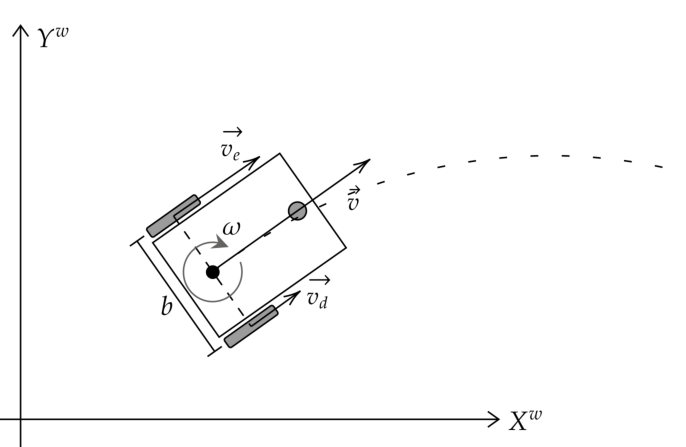
\includegraphics[trim=0 0 65 0, clip, width=\textwidth]{img/wheels_differential_speeds_crop.pdf}
        \caption{Esquema de velocidades do robô diferencial}
        \label{fig:Diff_Wheel_Velocities}
    \end{subfigure}
    \hspace{0.05\textwidth}
    \begin{subfigure}[b]{0.4\textwidth}
        \centering
        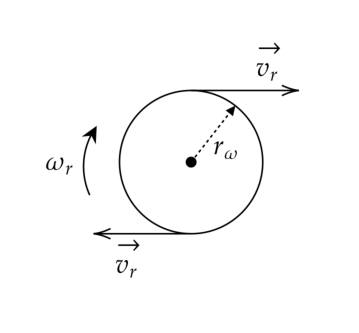
\includegraphics[width=0.7\textwidth]{img/wheel_speed_details_crop.pdf}
        \caption{Detalhe das velocidades das rodas do robô}
        \label{fig:Diff_Wheel_Detail}
    \end{subfigure}
    \source
    \label{fig:Diff_Wheel}
\end{figure}
    
    No ponto de controle definido, quando as rodas em lados opostos giram na mesma direção, o robô se move para frente com uma velocidade linear $(v)$. Se as rodas giram com velocidades de rotação diferentes, o robô desenvolve uma velocidade angular $(\omega)$. Essas velocidades podem ser expressas em termos das rotações das rodas esquerda $(\omega_e)$ e direita $(\omega_d)$ do robô.
    
    As velocidades linear $(v)$ e angular $(\omega)$  do ponto de controle podem ser obtidas pela média das velocidades exercidas por cada roda. Seja $\omega_E$ a velocidade angular do robô devido à roda esquerda e $\omega_D$ a velocidade angular devido à roda direita e definindo o sentido horário de movimento como positivo, teremos:

    \begin{eqnarray}
        v = \frac{v_e + v_d}{2} \qquad  \qquad \omega = \frac{\omega_E - \omega_D}{2}   \\
        v = \frac{v_e + v_d}{2} \qquad  \qquad \omega = \frac{\frac{v_e}{b/2} - \frac{v_d}{b/2}}{2}
    \end{eqnarray}
    
    % \begin{equation}
    %     v = \frac{v_e + v_d}{2}, \quad \omega = \frac{\frac{2v_e}{b} - \frac{2v_d}{b}}{2}
    % \end{equation}
    
    % \begin{equation}
    %     v = \frac{v_e + v_d}{2}, \quad \omega = (\frac{\cancel{2}v_e}{b} - \frac{\cancel{2}v_d}{b})\cdot\frac{1}{\cancel{2}}
    % \end{equation}

    Simplificando, obtemos:

    \begin{equation}
        v = \frac{v_e + v_d}{2} \qquad \text{e} \qquad \omega = \frac{v_e-v_d}{b}
    \end{equation}
    
    e com base na Figura \ref{fig:Diff_Wheel_Detail}, obtém-se as velocidades do robô em função das rotações das rodas esquerda e direita como:
    
    \begin{equation} 
    v = \frac{(\omega_e + \omega_d)r_w}{2} \qquad \text{e} \qquad \omega = \frac{(\omega_e - \omega_d)r_w}{b}, 
    \end{equation} 
    
    onde $r_w$ é o raio da roda e $b$ é a distância entre as rodas de um lado e as do outro \cite{Bouzoualegh2018ModelRobot} \cite{book:siegwart2011} \cite{Sarcinelli-Filho2023KinematicModels}.

    Para controlar as rotações das rodas esquerda e direita, sinais PWM são enviados para os controladores eletrônicos de velocidade (ESCs) montados em cada um dos motores. No entanto, a maioria dos robôs móveis podem ser controlados por sinais de controle de alto nível (comandos de velocidade linear e angular), a saber $ \bs{u} = \begin{bmatrix} v & \omega \end{bmatrix}^T $. Isso é possível pois os fabricantes implementam o controlador de baixo nível a bordo do veículo, que gera os sinais de controle PWM para mover as rodas a partir das velocidades de entrada e do modelo da dinâmica do veículo. Isso permite o controle das velocidades linear e angular do veículo usando sinais de controle de alto nível, com perda de desempenho mínima para movimentos de baixa aceleração. Portanto, para controlar o robô diferencial somente é necessário definir os comandos de velocidades linear e angular que este deve executar.

    % Para definir o controlador cinemático, utilizaremos o modelo de cinemática extendida do robô diferencial, pois este modelo permite o controle de qualquer ponto...
    O controlador utilizado neste trabalho é obtido pela técnica de cinemática inversa \cite{Sarcinelli-Filho2023_4}. Para utilizá-la, é necessário obter o modelo cinemático de um robô diferencial terrestre de modo que o ponto de controle não tenha restrições holonômicas e possa desenvolver velocidades nos dois eixos de referência do robô ($X^r$ e $Y^r$) \cite{Sarcinelli-Filho2023_2}. Com base na Figura \ref{fig:differential_mode}, podemos obter este modelo a partir das relações trigonométricas entre o referencial inercial do mundo e o referencial do robô, utilizando como ponto de controle o ponto $\bs{x}_c$, deslocado longitudinalmente do ponto $\bs{x}$.
    
    \begin{figure}[htb]
        \centering
        \caption{Cinemática 2D de um robô diferencial, mostrando a parte frontal do robô. A posição do robô, $ \bs{x} $, é deslocada por um valor \( a \). Isso resulta em um novo vetor de posição \( \bs{x}_c \), uma mudança que simplifica a implementação do controlador cinemático.}
        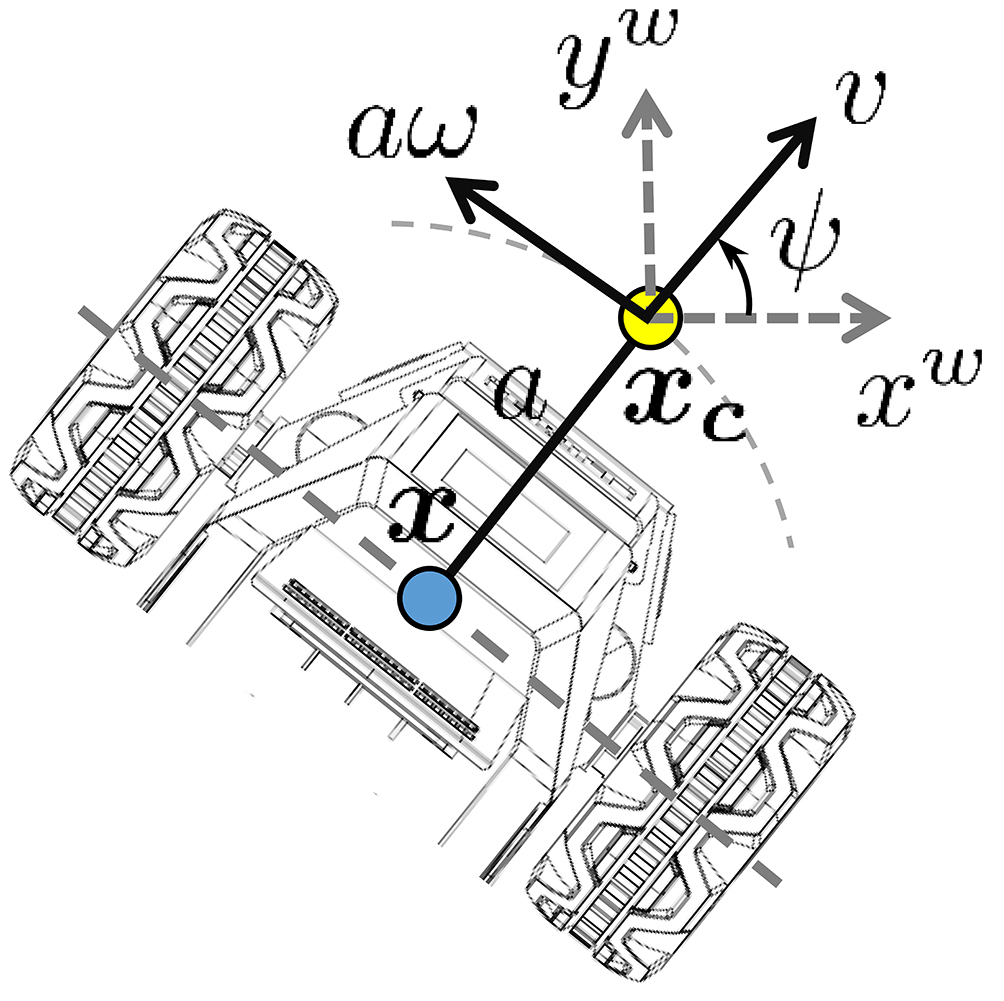
\includegraphics[width=0.4\linewidth]{limo_diff.jpg} 
        \label{fig:differential_mode}
        \source
    \end{figure}
    
    As relações entre as velocidades $v$ e $w$ do robô e as velocidades correspondentes no eixo inercial do mundo serão:
    
    \begin{align}
        \dot{x}_c &= v\cos{\psi} - a\omega\sin{\psi}   \\
        \dot{y}_c &= v\sin{\psi} + a\omega\cos{\psi}    \\
        \dot{\psi} &= \omega
    \end{align}

    que em notação matricial, fica:

    \begin{equation}
        \begin{bmatrix} \dot{x}_c \\ \dot{y}_c  \end{bmatrix} = \begin{bmatrix} \cos{\psi} & -a \sin{\psi} \\ \sin{\psi} & a \cos{\psi}   \end{bmatrix} \cdot \begin{bmatrix} v \\ \omega    \end{bmatrix}
        \label{eq:kinematics_differential}
    \end{equation}
    
    ou seja, \( \dot{\bs{x}}_c = \bs{H} \bs{u} \), em que $\bs{H}$ é a matriz de cinemática do robô diferencial \cite{Sarcinelli-Filho2023_2}. Note que esta matriz é invertível, o que permite obter a equação para o controlador utilizando a técnica de cinemática inversa \cite{Sarcinelli-Filho2023_4}, de tal forma que $\bs{u} = \bs{H}^{-1} \dot{\bs{x}}_{c,ref}$, ou, 
    
    \begin{align}
        \label{eq:kinematic_controller_differential}
        \dot{\bs{u}} \ \  & = \qquad \;  \bs{H}^{-1} \quad\;\; \cdot \; \; \bs{x}_{c\,ref}    \notag \\
        \begin{bmatrix} v \\ \omega    \end{bmatrix} & =  \begin{bmatrix} c_\psi & s_\psi \\ -\frac{1}{a}s_\psi & \frac{1}{a} c_\psi   \end{bmatrix} \cdot \begin{bmatrix}\dot{x}_{c,ref} \\ \dot{y}_{c,ref}   \end{bmatrix}
    \end{align}
    
   onde $ c(\cdot) $ e $ s(\cdot) $ representam as funções $ cosseno() $ e $ seno() $, respectivamente.
    
    A velocidade de referência \( \dot{\bs{x}}_{c,ref} \) é uma lei de controle de \textit{feedforward} e \textit{feedback} proporcional, tal que
    
    \begin{equation}
        \dot{\bs{x}}_{c,ref} = \dot{\bs{x}}_{c,des} + \bs{\kappa}(\bs{x}_{c,des} - \bs{x}_c),
        \label{eq:ff_fb_law}
    \end{equation}
    
    \noindent para o qual \( \bs{\kappa} \) é a matriz de ganhos do controlador, que deve ser uma matriz diagonal definida positiva.

    % \subsection{Controle de Robôs Diferenciais}
    % \label{sec:Controle_Robos_Diferenciais}

    
% \begin{itemize} 
%     \item \add{Controle de Posicionamento}
%     \item \add{Seguimento de Trajetória}
% \end{itemize}    

\section{Localização e Mapeamento Simultâneos}

No contexto da robótica móvel, o problema de Localização e Mapeamento Simultâneos (SLAM, do inglês \textit{Simultaneous Localization and Mapping}) surge como um dos desafios fundamentais para a autonomia de robôs. Em essência, o robô precisa construir um mapa de um ambiente desconhecido ao mesmo tempo em que estima sua própria pose (posição e orientação) dentro desse mapa \cite{Thrun2005}. Trata-se de uma tarefa complexa pois, diferentemente da simples localização com mapa previamente conhecido ou do mapeamento com pose conhecida, no SLAM tanto o mapa quanto a pose são inicialmente desconhecidos e precisam ser estimados\cite{Thrun2005}. 

Nas últimas décadas, pesquisas em SLAM alcançaram progressos notáveis, viabilizando aplicações em larga escala e até sua transição para setores industriais \cite{Yue2024} \cite{Cadena2016}. Ainda assim, o SLAM permanece um problema em aberto em muitos aspectos, especialmente devido a seus principais desafios práticos: a presença de incertezas significativas nas medições sensoriais e nos movimentos do robô, a necessidade de identificar fechamentos de ciclo de forma confiável, e a correta associação de dados sensoriais a elementos do mapa \cite{Yue2024} \cite{Placed2023AFrontiers} \cite{Bavle2023FromSurvey}.

A incerteza inerente aos sensores e à odometria faz com que erros se acumulem ao longo do deslocamento do robô, exigindo técnicas robustas para manter a estimativa consistente. Para isso, é necessário a detecção de fechamentos de ciclo (\textit{loop closure}), que consiste em detectar quando o robô retorna a uma região já mapeada – crucial para corrigir desvios acumulados no mapa e na pose \cite{Labbe2014}, o que depende de técnicas de associação de dados a fim de determinar quais observações correspondem a quais características do mapa (ou a novos marcos), evitando correspondências equivocadas que poderiam degradar o mapa \cite{Cadena2016}.

Diversos algoritmos foram propostos para tentar solucionar o problema de SLAM, combinando conceitos de robótica probabilística e otimização \cite{Thrun2005}\cite{Cadena2016}. A seguir são apresentados os principais tipos de algoritmos de SLAM, com uma breve descrição de cada um e suas características.

    \subsection{Tipos de Algoritmos de SLAM}
    
    Ao longo do desenvolvimento do SLAM, diferentes abordagens baseadas em estimadores Bayesianos e em técnicas de otimização foram exploradas. Entre os tipos mais influentes estão algoritmos baseados em filtro de Kalman estendido(EKF, do inglês \textit{Extended Kalman Filter}), em filtros de partículas e em grafos de otimização. Cada categoria apresenta formas distintas de representar e estimar o mapa e a pose do robô, com vantagens e limitações específicas, conforme descrito a seguir.
    
        \subsubsection{EKF-SLAM}
        
        Uma das abordagens clássicas para o SLAM é o \textbf{EKF-SLAM}, que emprega um Filtro de Kalman Estendido para estimar iterativamente o estado do robô e do mapa \cite{Thrun2005}. Nessa formulação, o estado mantido pelo filtro inclui a pose atual do robô e as posições estimadas de todos os marcos (landmarks) mapeados no ambiente. 
        
        O EKF propaga uma distribuição Gaussiana conjunta sobre este vetor de estado, atualizando um grande vetor de média e uma matriz de covariância a cada movimento executado (etapa de previsão) e a cada nova observação sensorial (etapa de correção) \cite{Thrun2005}. Intuitivamente, o EKF-SLAM começa sem nenhum marco conhecido; conforme o robô explora o ambiente e detecta novos marcos, estes são adicionados ao estado, e tanto a localização do robô quanto as posições dos marcos são refinadas. O filtro lineariza as funções não-lineares de movimento e percepção em torno do estado estimado (base do EKF), permitindo calcular a atualização de forma analítica, porém aproximada \cite{Thrun2005}. 
        
        A principal vantagem dessa abordagem é fornecer diretamente uma estimativa estatística completa (média e incerteza) tanto da pose quanto do mapa, capturando as correlações entre todas as variáveis. Isso permite, por exemplo, que o robô avalie quantitativamente sua incerteza de localização ao decidir seus próximos movimentos, tornando o sistema mais consciente de suas limitações. Entretanto, o EKF-SLAM apresenta alto custo computacional: a cada passo de atualização, a complexidade tende a crescer quadraticamente com o número de marcos mapeados, pois a matriz de covariância cresce com o quadrado do número de variáveis (pose + marcos), tornando a atualização cada vez mais custosa à medida que o mapa cresce. \cite{Thrun2005}. Isso restringe a escalabilidade para mapas grandes ou muito detalhados. Além disso, o método assume erros gaussianos e pequenas não-linearidades; em cenários de forte não-linearidade ou ambientes com marcos muito similares (causando ambiguidades), o EKF pode produzir estimativas inconsistentes ou até divergir \cite{Thrun2005}. A associação de dados, em particular, torna-se crítica: o EKF-SLAM geralmente utiliza a correspondência de máxima verossimilhança incremental para parear observações com marcos existentes, o que impede a revisão de associações passadas \cite{Thrun2005}. Uma má associação de dados (por exemplo, confundir dois marcos semelhantes) propaga erro sem possibilidade de revisão posterior, diferente de métodos baseados em grafos, como Graph-SLAM, que permitem reotimizar o mapa a posteriori. 

% \begin{algorithm}[H]
%     \caption{Algoritmo genérico para o EKF-SLAM}
%     \alg
%     \SetAlgoLined
%     \FuncSty{EKF\_SLAM(}\ArgSty{pose_anterior}) \
%         initialization\;
%     \While{not at end of this document}{
%         read current\;
%     \eIf{understand}{
%         go to next section\;
%         current section becomes this one\;
%     }{
%         go back to the beginning of current section\;
%     }
%     \If{$\Delta$ == true}{
%         show the match}
%     }

% \end{algorithm} 
        
        \subsubsection{FastSLAM – SLAM usando Filtro de Partículas}
        
        Para contornar algumas das limitações do EKF-SLAM, foi introduzido o \textit{FastSLAM}, uma família de algoritmos que aplicam filtros de partículas ao problema de SLAM \cite{Montemerlo2002} \cite{Thrun2005}. O FastSLAM explora a técnica de fatoração do problema de SLAM através de um filtro de partículas Rao-Blackwellizado. A ideia central é separar (matematicamente, fatorar) a estimativa da trajetória do robô da estimativa do mapa, aproveitando a independência condicional dos marcos (\textit{Landmarks}) quando a trajetória do robô é conhecida \cite{Montemerlo2002}. Em prática, o algoritmo mantém um conjunto de partículas, onde cada partícula representa uma hipótese para a trajetória percorrida pelo robô (sequência de poses estimadas) e possui seu próprio mapa associado (estimativas dos marcos) \cite{Thrun2005}. Dentro de cada partícula, as posições dos marcos são estimadas de forma local, tipicamente usando pequenos filtros de Kalman individuais para cada marco. Dessa forma, o filtro de partículas lida com a incerteza global da trajetória, enquanto os filtros locais (um por marco) lidam com a incerteza das posições dos marcos dada a trajetória conhecida. Essa abordagem fatorada reduz drasticamente a necessidade de manter e atualizar uma grande matriz de covariância conjunta, o que melhora a escalabilidade: a complexidade de atualização cresce linearmente com o número de marcos (multiplicado pelo número de partículas), em vez de quadraticamente \cite{Thrun2005}. Em muitas aplicações, um conjunto relativamente pequeno de partículas (dezenas a centenas) é suficiente para obter bons resultados, tornando o FastSLAM capaz de mapear ambientes maiores sem explosão do custo computacional. 
        
        O algoritmo FastSLAM original (às vezes chamado de FastSLAM 1.0) foi apresentado por Montemerlo et al. (2002) utilizando amostragem de partículas conforme a distribuição de movimento do robô, e posteriormente aprimorado no FastSLAM 2.0 com técnicas de amostragem mais informativas para melhorar a precisão \cite{Montemerlo2002}. Uma das grandes vantagens do FastSLAM é sua robustez em cenários onde o EKF-SLAM enfrentaria problemas de não-linearidade ou multi-modalidade na distribuição de probabilidade: o conjunto de partículas pode, teoricamente, representar hipóteses múltiplas sobre a pose do robô (por exemplo, diferentes posicionamentos caso o robô se localize em locais parecidos), coisa que um único filtro gaussiano não consegue fazer. Além disso, o FastSLAM permite incorporar facilmente observações com associações de dados diferentes em partículas distintas – ou seja, diferentes partículas podem “apostar” em associações de dados alternativas, mitigando em parte o risco de um erro de correspondência arruinar todo o mapa \cite{Thrun2005}. Entretanto, o FastSLAM também tem desvantagens. Uma delas é que, apesar de não manter explicitamente uma matriz de covariância completa, ele pode degradar em performance se o número de partículas necessário for alto – por exemplo, em ambientes muito extensos ou após longos percursos sem fechamento de ciclo, pode ser preciso um grande número de partículas para manter a consistência, o que aumenta o custo computacional e de memória. Outro ponto é que o erro de trajetória do robô (contido nas partículas) pode crescer ao longo do tempo; se poucas partículas sobreviverem representando corretamente a distribuição verdadeira da pose, o filtro de partículas pode sofrer de degeneração (perda de diversidade), tornando difícil recuperar um fechamento de ciclo tardio caso as partículas restantes não estejam próximas da solução correta \cite{Thrun2005}. Em outras palavras, o FastSLAM tende a tratar as correlações entre marcos de forma implícita via as partículas e, se essa representação implícita for insuficiente, podem ocorrer inconsistências, especialmente no momento de grandes fechamentos de loop \cite{Thrun2005}. Ainda assim, na prática, o FastSLAM mostrou-se muito eficaz e foi durante um período a técnica de estado da arte, sendo capaz de mapear trajetórias de quilômetros com precisão comparável a dos métodos de filtro gaussiano tradicionais, porém com melhor escalabilidade \cite{Thrun2005}. Esse método abriu caminho para SLAM em tempo real com veículos autônomos e robôs de serviço em ambientes maiores, e influenciou também algoritmos modernos de mapeamento baseados em grades de ocupação (ocupancy grids) e SLAM visual que empregam partículas ou múltiplas hipóteses \cite{Thrun2005}.

        
        \subsubsection{SLAM Baseado em Grafos}
        
        Nos últimos anos, a abordagem dominante para SLAM tem se voltado aos métodos baseados em grafos, também conhecidos como \textit{Graph-Based SLAM} ou \textit{GraphSLAM} \cite{Grisetti2010}\cite{Labbe2014}. Diferentemente das abordagens discutidas anteriormente, que utilizam filtros sequenciais (a estimativa de pose atual é dependente das estimativas anteriores), o SLAM baseado em grafos formula o problema como uma otimização global: constrói-se um grafo de variáveis que representa o histórico de poses do robô (cada nó no grafo é uma pose do robô em um determinado instante, ou alternativamente, um marco mapeado, dependendo da formulação) e as medições são representadas por arestas que conectam os nós, impondo restrições espaciais entre poses (ou entre pose e marco) \cite{Labbe2014}. Por exemplo, a odometria do robô introduz arestas conectando cada pose com a pose seguinte, enquanto uma observação de um marco visto em duas poses diferentes gera uma aresta de restrição entre essas poses (ou entre pose e nó de marco). O objetivo então é encontrar os valores de todas as poses (e eventualmente das coordenadas dos marcos) que melhor satisfazem todas as restrições do grafo – tipicamente formulado como um problema de mínimos quadrados não-lineares, resolvido por métodos de otimização iterativa (como Gauss-Newton, Levenberg-Marquardt, etc.) \cite{Zhang2021}. Em essência, o Graph-SLAM procura a configuração de mapa e trajetória com máxima consistência global, em vez de atualizar as estimativas de pose incrementalmente a cada iteração do algoritmo.
        
        A vantagem clara dessa formulação é que ela lida de forma natural com o fechamento de ciclo e com múltiplas restrições redundantes. Quando o robô detecta um lugar previamente visitado (loop closure), adiciona-se uma nova aresta no grafo conectando as poses correspondentes; a otimização do grafo então ajusta todas as poses de maneira coerente para acomodar essa nova informação, distribuindo o erro acumulado pelo laço fechado \cite{Labbe2014}. Diferentemente do EKF, que propagava correlações de maneira implícita e incremental, o grafo torna explícitas as relações entre poses e permite recalcular o mapa inteiro de forma consistente ao encontrar novas relações. Além disso, a estrutura esparsa do problema (cada medida relaciona apenas algumas variáveis) pode ser explorada para eficiência: técnicas de otimização de grafos conseguem resolver mapas com milhares de poses e restrições em tempo real ou próximo de tempo real, algo impraticável para um EKF que manteria um gigantesco vetor de estado denso \cite{Grisetti2010}. Na literatura, diversos frameworks de otimização de grafos foram desenvolvidos para SLAM, como por exemplo \textit{iSAM}, \textit{g2o}, entre outros, que aplicam estratégias de linearização incremental e fatoração matricial aproveitando a esparsidade das jacobianas \cite{Juric2021ASLAM} \cite{Kummerle2017G2o:Optimization} \cite{Kaess2008ISAM:Mapping} \cite{Li2021Gumbel-softmax-basedGraphs}. Como resultado, o SLAM baseado em grafos tornou-se a espinha dorsal de muitos sistemas modernos de mapeamento. Por exemplo, algoritmos de SLAM visual de última geração tipicamente mantêm um grafo de poses de câmera (frequentemente chamadas de keyframes) e realizam otimizações globais conhecidas como \textit{bundle adjustment} ou otimização de \textit{pose graph} para minimizar a reprojeção de pontos no mapa \cite{MurArtal2017}\cite{Zhang2021}. No caso de SLAM com sensores RGB-D ou LiDAR, também é comum construir um grafo de poses onde cada aresta representa a correspondência entre nuvens de pontos ou características visuais detectadas entre duas poses, e então um otimizador distribui os erros ao longo do grafo \cite{Zhang2021}. 
        
        Um ponto importante do SLAM por grafo é a separação conceitual entre o \textit{front-end} e o \textit{back-end} do sistema. O \textit{front-end} é responsável por processar os dados brutos dos sensores para extrair informações relevantes (por exemplo, detectar feições visuais ou geometrias em um laser) e por tomar decisões de associação de dados e detecção de fechamentos de loop – ou seja, construir as arestas do grafo de forma correta. Já o \textit{back-end} pega esse grafo de restrições construído e realiza a otimização matemática para ajustar as estimativas de pose/mapa \cite{Cadena2016}. Essa modularidade permite incorporar técnicas avançadas de reconhecimento de lugares (como detecção de loop closures baseada em visão, descritores de imagem, etc) sem modificar o núcleo do estimador, e vice-versa, possibilitando aplicar algoritmos de otimização genéricos independentemente do tipo de sensor utilizado \cite{Labbe2014}. Entretanto, o desempenho do Graph-SLAM depende criticamente da qualidade do front-end: associações de dados incorretas podem degradar a solução se não forem tratadas, exigindo esquemas robustos para rejeitar \textit{outliers} ou usar funções de perda robusta na otimização. Ainda assim, a abordagem de grafo é atualmente considerada o estado da arte em SLAM devido à sua precisão e flexibilidade. Estudos e sistemas recentes confirmam sua eficácia em cenários reais complexos, incluindo mapeamento de longo prazo e multi-sessão \cite{Labbe2014}, SLAM visual e RGB-D em larga escala \cite{MurArtal2017} \cite{Zhang2021}, entre outros.

        Como demonstrado por \citeonline{Labbe2014}, a detecção confiável de fechamentos de ciclo em um SLAM gráfico de larga escala pode lidar até com cenários de mapeamento multi-sessão, nos quais o robô pode ser reinicializado em locais diferentes e ainda assim unificar os mapas através de correspondências encontradas posteriormente. Assim, o SLAM baseado em grafos oferece uma solução elegante e eficaz para o problema de localização e mapeamento simultâneos, motivo pelo qual foi adotado neste projeto.
        
        Vale destacar que o presente trabalho utiliza um método de SLAM baseado em grafos, a \textbf{SLAM Toolbox} \cite{site:Slam_toolbox}. Optou-se pela utilização desta biblioteca de SLAM robusta e amplamente testada, presente no ecossistema ROS (Robot Operating System). A utilização desta biblioteca é recomendada nos tutoriais de SLAM do pacote Nav2 do ROS 2, o pacote padrão utilizado para navegação de robôs, demonstrando a confiança da comunidade ROS nesta biblioteca. 